\documentclass [letterpaper,11pt,twoside] {article}
%\usepackage{pst-pdf,pst-text,pstricks-add}
\providecommand{\ifincludeall}{\iffalse}
\usepackage{fancyhdr}
\usepackage{lastpage}
\usepackage{enumerate}
\ifincludeall

  \usepackage{wrapfig}

%================================ Unicode ================================
  \usepackage[utf8]{inputenc}
  \DeclareUnicodeCharacter{916}{\ensuremath{\Delta}}
  \DeclareUnicodeCharacter{937}{\ensuremath{\Omega}}
  \DeclareUnicodeCharacter{949}{\ensuremath{\epsilon}}
  \DeclareUnicodeCharacter{956}{\ensuremath{\mu}}
  \DeclareUnicodeCharacter{963}{\ensuremath{\sigma}}
  \DeclareUnicodeCharacter{977}{\ensuremath{\theta}}
  \DeclareUnicodeCharacter{1009}{\ensuremath{\rho}}
  \DeclareUnicodeCharacter{03B4}{\ensuremath{\delta}}
  \DeclareUnicodeCharacter{221A}{\sqrt}
  \DeclareUnicodeCharacter{2124}{\ensuremath{\mathbb Z}}
%============================== End Unicode ==============================
\fi


\usepackage{amsmath}
\usepackage{amssymb}
%================================= AMSTHM =================================
\usepackage{amsthm}

\newtheorem{thm}{Theorem}[section]
%\newtheorem{theorem}{Theorem}
\newtheorem{conjecture}{Conjecture}[section]
\newtheorem{lem}{Lemma}[section]
%\newtheorem{lemma}[theorem]{Lemma}
\newtheorem{cor}[thm]{Corollary}
%\newtheorem{corollary}[theorem]{Corollary}
\newtheorem{prop}[thm]{Proposition}
%\newtheorem{proposition}[theorem]{Proposition}
%\newtheorem{definition}[theorem]{Definition}
%\newtheorem{example}[theorem]{Example}
\newtheorem{exercise}[thm]{Exercise}
%\newtheorem{exercise}[theorem]{Exercise}
\newtheorem{claim}[thm]{Claim}
\newtheorem{law}{Law}[section]
\newtheorem*{thm*}{Theorem}
\newtheorem*{lem*}{Lemma}
\newtheorem*{conjecture*}{Conjecture}
\newtheorem*{cor*}{Corollary}
\newtheorem*{prop*}{Proposition}
\newtheorem*{exercise*}{Exercise}
\newtheorem*{law*}{Law}
\newtheorem*{claim*}{Claim}



\theoremstyle{definition} \newtheorem{defn}{Definition}[section]
\theoremstyle{definition} \newtheorem*{defn*}{Definition}
\newtheorem{example}[thm]{Example}
\newtheorem*{example*}{Example}
\newtheorem{eg}[thm]{Example}
\newtheorem*{eg*}{Example}

\newtheorem{fact}{Fact}[section]
\newtheorem*{fact*}{Fact}

\newcommand{\thmref}[1]{Theorem~\ref{#1}}
%=============================== End AMSTHM ===============================
\usepackage{esint}
\ifincludeall
  \usepackage[table]{xcolor}
  \usepackage{xifthen}
\fi
%\if dcpic
%\usepackage{dcpic}
%\else

%\ifincludeall
  \usepackage{ifpdf}
%\else
  %\newif\ifpdf
  %\pdftrue
%\fi

\ifincludeall
  \ifpdf
    \usepackage[pdftex]{graphicx}
    \usepackage{pdfpages}
    \usepackage[plainpages=false,pdfpagelabels,unicode]{hyperref}
  \else
    \usepackage[dvips]{graphicx}
    \usepackage{pstricks,pstricks-add,pst-math,pst-xkey}
  \fi
\else
  \usepackage[pdftex]{graphicx}
  \usepackage[pdfpagelabels,unicode]{hyperref}
\fi

%\ifincludeall
  \usepackage{mathtools}
%\fi

%\global\def\isxy{}
%\global\let\isxy\relax
\ifincludeall
  \providecommand{\isxy}{\let\isxy\relax}
  \expandafter\ifx\isxy\relax
    %\usepackage{mathpazo} or \usepackage{mathptmx} 
    \usepackage{flexisym} % flexisym package is required by breqn
                          % can load as \usepackage[mathpazo]{flexisym}
    \usepackage{breqn}
  \else
    \usepackage[all]{xy}
  \fi
\fi



%\usepackage[exponent-product=\cdot,per-mode=fraction,quotient-mode=fraction,fraction-function=\sfrac]{siunitx} %alsoload={named,prefixed,abbr,hep},
%\newunit{\statvolt}{statV}
%\newunit{\erg}{erg}
%\newunit{\esu}{esu}

\providecommand{\abs}[1]{\left\lvert#1\right\rvert}%\DeclarePairedDelimiter\abs{\lvert}{\rvert} %\providecommand{\abs}[1]{\lvert#1\rvert}
\ifincludeall
  \DeclarePairedDelimiter\norm{\lVert}{\rVert}
  \DeclarePairedDelimiter\floor{\lfloor}{\rfloor}
\else
  \providecommand{\floor}[1]{\left\lfloor #1\right\rfloor}
  \providecommand{\norm}[1]{\lVert#1\rVert}
\fi
\newcommand{\gcdf}[2]{\left( #1 , #2 \right)}
\DeclareMathOperator{\lcm}{lcm}
\DeclareMathOperator{\im}{im}
\DeclareMathOperator{\rank}{rank}
\DeclareMathOperator{\spans}{span}
\DeclareMathOperator{\divergence}{div}
\DeclareMathOperator{\tr}{tr}
\DeclareMathOperator{\grad}{grad}
\DeclareMathOperator{\spec}{Spec}
\DeclareMathOperator{\pspec}{PSpec}
\DeclareMathOperator{\rad}{rad}
\DeclareMathOperator{\trdeg}{tr\,deg}
\DeclareMathOperator{\gk}{gk}
\DeclareMathOperator{\fract}{fract}
\newcommand{\lcmf}[2]{\lcm\left( #1 , #2 \right)}
\def\dbar{{\mathchar'26\mkern-12mu d}}

\def\sfrac#1/#2{\leavevmode\kern.1em\raise.5ex\hbox{\the\scriptfont0 #1}\kern-.1em/\kern-.15em\lower.25ex\hbox{\the\scriptfont0 #2}}

\renewcommand{\d}{\,d}

\newcommand{\defeq}{\coloneqq}%\stackrel{\mathrm{df}}{=}}%{\ensuremath{:=}}%

\ifincludeall
  \newcommand{\complementset}[1][\ \ \rule{0pt}{1ex}]{\overline{#1}}
  \newcommand{\boldcomplementset}[1][\ \ \rule{0pt}{1ex}]{\text{\makebox[0pt][l]{$#1$}}\rule[\heightof{#1}+3pt]{\widthof{#1}}{0.11ex}}
  \let\oldboldsymbol=\boldsymbol
  \renewcommand{\boldsymbol}[1]{\let\oldcomplementset=\complementset%
  %\oldboldsymbol{#1}\  	%
  \let\complementset\boldcomplementset%
  \oldboldsymbol{#1}%
  \let\complementset=\oldcomplementset}
\fi
% \gdef\phantomhdepth{\relax}
% \gdef\phantomhdepth{1}
% \newcommand{\phantomheight}[1]{         %
% \ifx\phantomhdepth\relax          %
%   \let\phantomhdepth{1}          %
%   \vphantom{#1}          %
%   \let\phantomhdepth\relax          %
% \fi          %
% }
\newcommand{\tuple}[1]{\breakingtuple{#1}}
\newcommand{\nbtuple}[1]{\left(#1\right)}
\newcommand{\breakingtuple}[1]{\lrbreak{(}{#1}{)}}         %$
         %\let\oldcomma=,
\begingroup
  \lccode`~=`,
  \lowercase{\endgroup
    \let\oldcomma=~
    \def\comma{\oldcomma}
    \def~{\comma}         %
  }         %
         %\def\aaa{\comma}
         %\mathcode`,="613B

\newcommand{\allowbreaks}[1]{\begingroup \mathcode`,="8000 \def\comma{\oldcomma\allowbreak}#1\def\comma{\oldcomma} \mathcode`,="613B \endgroup }         %\replace{#1}{,}{,\allowbreak}}
%\let\phantomheight\vphantom
\newcommand{\lbreakh}[4][\!\!]{\left#2\vphantom{#3#4}\right.#1\allowbreaks{#3}}
\newcommand{\rbreakh}[4][\!\!]{#2#1\left.\vphantom{#2#4}\right#3}
\newcommand{\lrbreakh}[5][\!\!]{\left#2\vphantom{#3#5}\right.#1\allowbreaks{#3}#1\left.\vphantom{#3#5}\right#4}
\newcommand{\lbreak}[3][\!\!]{\lbreakh[#1]{#2}{#3}{}}
\newcommand{\rbreak}[3][\!\!]{\rbreakh[#1]{#2}{#3}{}}
\newcommand{\lrbreak}[4][\!\!]{\lrbreakh[#1]{#2}{#3}{#4}{}}
\newcommand{\olrbreak}[5][\!\!]{\overlineb{\lrbreakh[#1]{#2}{#3}{.}{#4}}{\lrbreakh[#1]{.}{#4}{#5}{#3}}}
\newcommand{\olrbreakc}[6][\!\!]{\overlineb{#2\lbreakh[#1]{#3}{#4}{#5}}{\rbreakh[#1]{#5}{#6}{#4}}}%\lrbreak[#1]{.}{#5}{#5}}}

%\DeclarePairedDelimiter\simpleset{\lbrace}{\rbrace}
\newcommand{\simpleset}[1]{\left\lbrace#1\right\rbrace}
\newcommand{\simplesetb}[1]{\lrbreak{\lbrace}{#1}{\rbrace}}

\newcommand{\mathsetb}[2][\relax]{%
\ifx#1\relax
  \simplesetb{#2}
\else
  \simplesetb{\suchthatb[#1]{#2}}
\fi}

\newcommand{\mathset}[2][\relax]{%
\ifx#1\relax
  \simpleset{#2}
\else
  \simpleset{\suchthat[#1]{#2}}
\fi}
\newcommand{\omathset}[3][\relax]{%
\ifx#1\relax
  \overlineb{\lrbreak{\lbrace}{#2}{.}}{\lrbreak{.}{#3}{\rbrace}}
\else
  \overlineb{\lrbreak{\lbrace}{\suchthat[#1]{#2}}{.}}{\lrbreak{.}{#3}{\rbrace}}
\fi}

\newcommand{\omathsetc}[4][\relax]{%
\ifx#1\relax
  \overlineb{\lrbreak{\lbrace}{\suchthat[#2]{#3}}{.}}{\lrbreak{.}{#4}{\rbrace}}
\else
  \overlineb{#1\lrbreak{\lbrace}{\suchthat[#2]{#3}}{.}}{\lrbreak{.}{#4}{\rbrace}}
\fi}
  
\newcommand{\overlinet}[2]{\overlineb{#1}{#2}}
\newcommand{\overlineb}[2]{\overline{#1\vphantom{#2}}\allowbreak\overline{#2\vphantom{#1}}}
%\newcommand{\overlinec}[3]{\overline{#1\text{\makebox[0pt]{$\phantom{#2#3}$}}}\allowbreak\overline{#2\vphantom{#1#3}}\allowbreak\overline{#3\vphantom{#1#2}}}

\newcommand{\suchthat}[2][]{#1\left\vert\vphantom{#1#2}\right.\!#2}
\newcommand{\suchthatb}[2][]{#1 \lbreakh[\!]{\vert}{#2}{#1}}
\providecommand{\scfont}{}

%texbook
%\newif\ifv@ \newif\ifh@
%\def\vphantom{\v@true\h@false\ph@nt}
%\def\hphantom{\v@false\h@true\ph@nt}
%\def\phantom{\v@true\h@true\ph@nt}
%\def\ph@nt{\ifmmode\def\next{\mathpalette\mathph@nt}%
%\else\let\next=\makeph@nt\fi \next}
%\def\makeph@nt#1{\setbox0=\hbox{#1}\finph@nt}
%\def\mathph@nt#1#2{\setbox0=\hbox{$\m@th#1{#2}$}\finph@nt}
%\def\finph@nt{\setbox2=\null \ifv@ \ht2=\ht0 \dp2=\dp0 \fi
%\ifh@ \wd2=\wd0 \fi \box2 }


%\def\m@th{\mathsurround=0pt }
\def\uncurry#1#2{#1#2} % \uncurry\macro1{{arg1}{arg2}...} -> \macro1{arg1}{arg2}...
\def\curryone#1#2#3{{\def\ndef{\noexpand\def}\def\first{\noexpand#1}\expandafter}\ifx\ndef\first #1{#2{#3}}\else #1{{#2}{#3}}\fi}
\def\currytwo#1#2#3#4{#1{{#2}{#3}{#4}}}
\def\currythree#1#2#3#4#5{#1{{#2}{#3}{#4}{#5}}}
\def\curryfour#1#2#3#4#5#6{#1{{#2}{#3}{#4}{#5}{#6}}}
\def\curryfive#1#2#3#4#5#6#7{#1{{#2}{#3}{#4}{#5}{#6}{#7}}}
\def\currysix#1#2#3#4#5#6#7#8{#1{{#2}{#3}{#4}{#5}{#6}{#7}{#8}}}
\def\curryseven#1#2#3#4#5#6#7#8#9{#1{{#2}{#3}{#4}{#5}{#6}{#7}{#8}{#9}}}


\def\uncurrytwo#1#2#3{#1#2#3}
\def\uncurriedmathpalette#1{\def\uncurried{\uncurrytwo#1}\mathpalette\uncurried}
\def\mathpalettetwo#1#2#3{\uncurriedmathpalette{#1}{{#2}{#3}}}
\def\mathpalettethree#1#2#3#4{\uncurriedmathpalette{#1}{{#2}{#3}{#4}}}


%\def\aswidthof{\v@false\h@true\@sof}
%\def\asheightof{\v@true\h@false\@sof}
%\def\assizeof{\v@true\h@true\@sof}

%\newcommand{\@sof}[3][l]{\ifmmode \def\next{\mathpalettethree\math@sof}%
%\else\let\next=\make@sof\fi \next{#1}{#2}{#3}}
%
%\def\make@sof#1#2#3{\setbox0=\hbox{#2}\setbox2=\makebox[0pt][c]{#3}\fin@sof}
%\def\math@sof#1#2#3{\setbox0=\hbox{$\m@th#1{#2}$}\setbox2=\hbox{$\m@th#1{#3}$}\fin@sof}
%\def\fin@sof{\ifv@ \ht2=\ht0 \dp2=\dp0 \fi
%\ifh@ \wd2=\wd0 \fi \box2 }
\makeatletter
\newcommand{\aswidthof}[3][c]{\ifmmode \def\next{\mathpalettethree\m@th@swidthof}%
\else\let\next=\m@ke@swidthof\fi \next{#1}{#2}{#3}}

\newdimen\@widthof
\newcommand{\m@th@swidthof}[4]{\text{\settowidth\@widthof{$\m@th#1#3$}\makebox[\@widthof][#2]{$\m@th#1#4$}}}
\newcommand{\m@ke@swidthof}[3]{\settowidth\@widthof{#2}\makebox[\@widthof][#1]{#3}}


%
%
%
%
%
%\makeatletter
%
%\def\aswidthof{\v@false\h@true\@sof}
%\def\asheightof{\v@true\h@false\@sof}
%\def\assizeof{\v@true\h@true\@sof}
%
%\def\@sof{\ifmmode\def\next##1##2{\mathpalette{\math@sof##1##2}}%
%\else\let\next=\make@sof\fi \next}
%
%\def\make@sof#1#2{\setbox0=\hbox{#1}\setbox2=\hbox{#2}\fin@sof}
%\def\math@sof#1#2#3{\setbox0=\hbox{$\m@th#3{#1}$}\setbox2=\hbox{$\m@th#3{#2}$}\fin@sof}
%\def\fin@sof{\ifv@ \ht2=\ht0 \dp2=\dp0 \fi
%\ifh@ \wd2=\wd0 \fi \box2 }

%\text{\newdimen\tempwidth \settowidth\tempwidth{$#3$}\makebox[\tempwidth][#1]{$#2$}}}% \text{\raisebox{0ex}[-\height][-\height]{$\phantom{#2}$}}}
%\newcommand{\asheightof}[3]{#1\text{\makebox[0pt]{$\phantom{#2}$}}\right.#2\left.\text{\makebox[0pt]{$\phantom{#2}$}}#3}

% 276887 sp is twice the width difference between $\left(\right)$ and $\left(\right.\left.\right)$
% \hspace{-138444 sp} \hspace{-138443 sp}\
\makeatletter
\def\breakingleft#1{{\def\templeft##1\breakingright##2{\left#1\vphantom{##1}\right.\n@space##1\n@space\left.\vphantom{##1}\right##2}\expandafter}\templeft}

\newcommand{\fullexpand}[2][]{{#1\edef\temp{#2}\expandafter}\temp}
\def\settoksexpanded#1=#2{{\edef\temp{{#2}}\expandafter}\expandafter#1\expandafter=\temp}

\newcommand{\selectfontsize}[1]{\fontsize{#1}{#1}\selectfont}

\newcommand{\newlinep}{$\left.\right.$\par\noindent}

\makeatletter
\newcommand{\interitemtext}[1]{%
\begin{list}{}
{\itemindent=0mm\labelsep=0mm
\labelwidth=0mm\leftmargin=0mm
\addtolength{\leftmargin}{-\@totalleftmargin}}
\item #1
\end{list}}
\makeatother


\newcommand{\ncr}[2]{\binom{#1}{#2}}
\newcommand{\definition}[1]{\begin{defn}#1\end{defn}}%{\par \noindent {\bf Definition:} #1}
\newcommand{\factc}[1]{\par \noindent \underline{\bf Fact:} #1}
%\providecommand{\lrang}[1]{\left\langle#1\right\rangle}%\DeclarePairedDelimiter\lrang{\langle}{\rangle}
\providecommand{\WLOG}{Without loss of generality}
\providecommand{\TFAE}{The following are equivalent}%{These facts are excellent}%(Ari)
\def\<#1>{\left\langle#1\right\rangle}
\def\[#1]{\left[#1\right]}
%\def\{#1|#2}{\mathset[#1]{#2}}
\providecommand{\End}[1]{\mathop{End}\left(#1\right)}
\providecommand{\dom}[1][\relax]{\mathop{dom}%
\ifx#1\relax%
\else%
  \left(#1\right)%
\fi}

\providecommand{\ses}{short exact sequence}
\providecommand{\st}{such that}


\newenvironment{digression}{\noindent\begin{math}%
\left(\ \begin{minipage}{0.95\textwidth}% FIX: Make this more robust
  }{\end{minipage}\ \right)\end{math}}

%\newenvironment{correction}{\textcolor{red}}{}
%======================================== Physics ===================================================
\providecommand{\uvec}[1]{{\widehat{\bf{#1}}}}
%\MakeAtOther
%\providecommand{\declareunits}[1][km,m,cm,mm,s,L,mL,kg,g]{%
%\@for\@unit:=#1\do{%
%  \declareunit{\@unit}%
%}}
%\providecommand{\declareunit}[2][\relax]{\ifx#1\relax%
%  \def\csname #2\endcsname{\text{#2}}%
%\else
%  \def\csname #1\endcsname{\text{#2}}%
%\fi}
%====================================================================================================

%================================= Proof Cases ===============================
\newcounter{ProofCasesLvlCtr}
\newcounter{ProofCasesMaxCtr}
\newcounter{ProofCasesCurCtr}
\newenvironment{proof-cases}[1][1]{%
\setcounter{ProofCasesCurCtr}{\value{ProofCasesLvlCtr}}%
\ifthenelse{\arabic{ProofCasesMaxCtr} = \arabic{ProofCasesLvlCtr}}{%
  \stepcounter{ProofCasesLvlCtr}%
  \stepcounter{ProofCasesMaxCtr}%
  \expandafter\newcounter{ProofCasesCtr\arabic{ProofCasesLvlCtr}}%
  \ifthenelse{\arabic{ProofCasesLvlCtr} = 1}{%
    \expandafter\edef\csname labelProofCases\arabic{ProofCasesLvlCtr}\endcsname{Case~\noexpand\arabic{ProofCasesCtr\arabic{ProofCasesLvlCtr}}}%
  }{%
    \expandafter\edef\csname labelProofCases\arabic{ProofCasesLvlCtr}\endcsname{\csname labelProofCases\arabic{ProofCasesCurCtr}\endcsname.\noexpand\arabic{ProofCasesCtr\arabic{ProofCasesLvlCtr}}}%
  }%
}{%
  \stepcounter{ProofCasesLvlCtr}%
  \ifthenelse{\arabic{ProofCasesLvlCtr} = 1}{%
    \expandafter\edef\csname labelProofCases\arabic{ProofCasesLvlCtr}\endcsname{Case~\noexpand\arabic{ProofCasesCtr\arabic{ProofCasesLvlCtr}}}%
  }{%
    \expandafter\edef\csname labelProofCases\arabic{ProofCasesLvlCtr}\endcsname{\csname labelProofCases\arabic{ProofCasesCurCtr}\endcsname.\noexpand\arabic{ProofCasesCtr\arabic{ProofCasesLvlCtr}}}%
  }%
}%
\begin{list}{\csname labelProofCases\arabic{ProofCasesLvlCtr}\endcsname:}{\expandafter\usecounter{ProofCasesCtr\arabic{ProofCasesLvlCtr}}}%
\expandafter\setcounter{ProofCasesCtr\arabic{ProofCasesLvlCtr}}{#1-1}%
}{\end{list}\addtocounter{ProofCasesLvlCtr}{-1}}
%\usepackage[pointlessenum]{paralist}
%\newenvironment{proof-cases}{\begin{enumerate}[{Case} 1:]}{\end{enumerate}}
%=============================== End Proof Cases =============================

\allowdisplaybreaks[1]

\usepackage [margin=1in]{geometry}

\def \d {\, {\rm d}}

\usepackage {wasysym}
\usepackage {pdfcomment}
\usepackage {cancel}
\usepackage [all]{xy}
\newcommand {\cheadcontent }{18.721 Notes}

\pagestyle {fancy}
\headheight 13.7pt
\fancyhead {}
\fancyhead {Jason Gross}\fancyfoot {}
\lhead {Jason Gross}
\rhead {\TeX ed on \today }
\chead {\cheadcontent }
\cfoot {\thepage \ of \pageref {LastPage}}
\begin {document}
\setcounter {section}{5}\section {Wednesday, February 16, 2011}
  \subsection{Plane curves}
    monomials $m_1, \ldots, m_N$, coefficients $z_1,\ldots, z_N$
    \begin{align*}
      Z & = \text{the space of all homogeneous polynomials of degree $d$ in $x$, $y$, and $z$} \\
        & = \text{affine space with coordinates $z_\nu$}
    \end{align*}
    (We have $f(x, y, z) = z_1x^d + z_2 x^{d-1} + \cdots$)

    $U = $ open subset in $Z$ corresponding to smooth plane curves

    $\mathcal C \subset \mathbb P^2 \times Z$

    $$
    \xymatrix{
    \mathcal C \ar[drr] & \subset & \mathbb P^2 \times Z \ar[d] && \mathcal C|_U = \mathcal C_U \ar[drr] & \subset & \mathbb P^2 \times U \ar[d] \\
                       &         &  Z                           && && U
    }
    $$

    \begin{prop*}
      Smooth plane curves are orientable and connected surfaces, and compact.
    \end{prop*}
    \begin{proof}
      Oreintability was done last time.

      To check connectedness, we just need to check one smooth curve of degree $d$ is connected.  $\mathcal C : \{ x^d + y^d - z^d = 0 \}$.

      Look at the line $y = z$.  On $U_2$, taking $z = 1$ we have $x^d + y^d = 1$.  Since $y = z$, $y = 1$, and then $x^d = 0$.  Since this is a root of order $d$, $C$ meets this line in only one point.  This means that it's connected. (WHY?)
    \end{proof}

    Given a connected, orientable, compact surface, it's topologically characterized by $g = \text{the genus} = \text{the \# of holes}$.

    \begin{defn*}
      The \emph{Euler characteristic} of $C$ is $2 - 2g$.
    \end{defn*}

    The Euler characteristic can be computed used an arbitrary triangulation, and then $E = \text{\# vertices} - \text{\# edges} + \text{\# faces}$.

    A sphere is, topologically, a tetrahedron, we have that the Euler characteristic is $4 - 6 + 4 = 2$.  We can do a similar thing for a torus.

    What is the Euler characteristic and genus of a smooth plane curve of degree $d$?

    Let's represent a smooth plane curve as a branched cover of $\mathbb P^1$.

    \begin{enumerate}[{Method }I]
      \item Start with the Fermat curve, and do an explicit calculation.  $C: \{x^d + y^d - z^d = 0\}$ \\
        Taking $z = 1$, $U_2 \simeq \mathbb A^2 \simeq \mathbb C^2$.  Then we have $x^d + y^d = 1$.  Drop $y$ by projection.
        Fix a value $x_0$ for $x$.  Then the line $y = x_0$ intersects the curve in $\le d$ points.
        Typically, we get $d$ values for $y$.
        \begin{enumerate}[{Case }I]
          \item $x_0^d \ne 1$.  Solve $y^d = 1 - x_0^d$.  There are $d$ solution s (if $y$ is a solution, then so is $yr^{2 \pi i j / d}$ for $0 \le j \le d$)
          \item $x_0^d = 1$.  Solve $y^d = 0$.  The only solution is $y = 0$. Now we look at $x_0$.  Triangulate $\mathbb P^1$, which is a sphere, as follows.  There are $d$ values for $x_0$, $x_i^d = 1$, $x_i = e^{2\pi i j / d}$.
      \begin{center}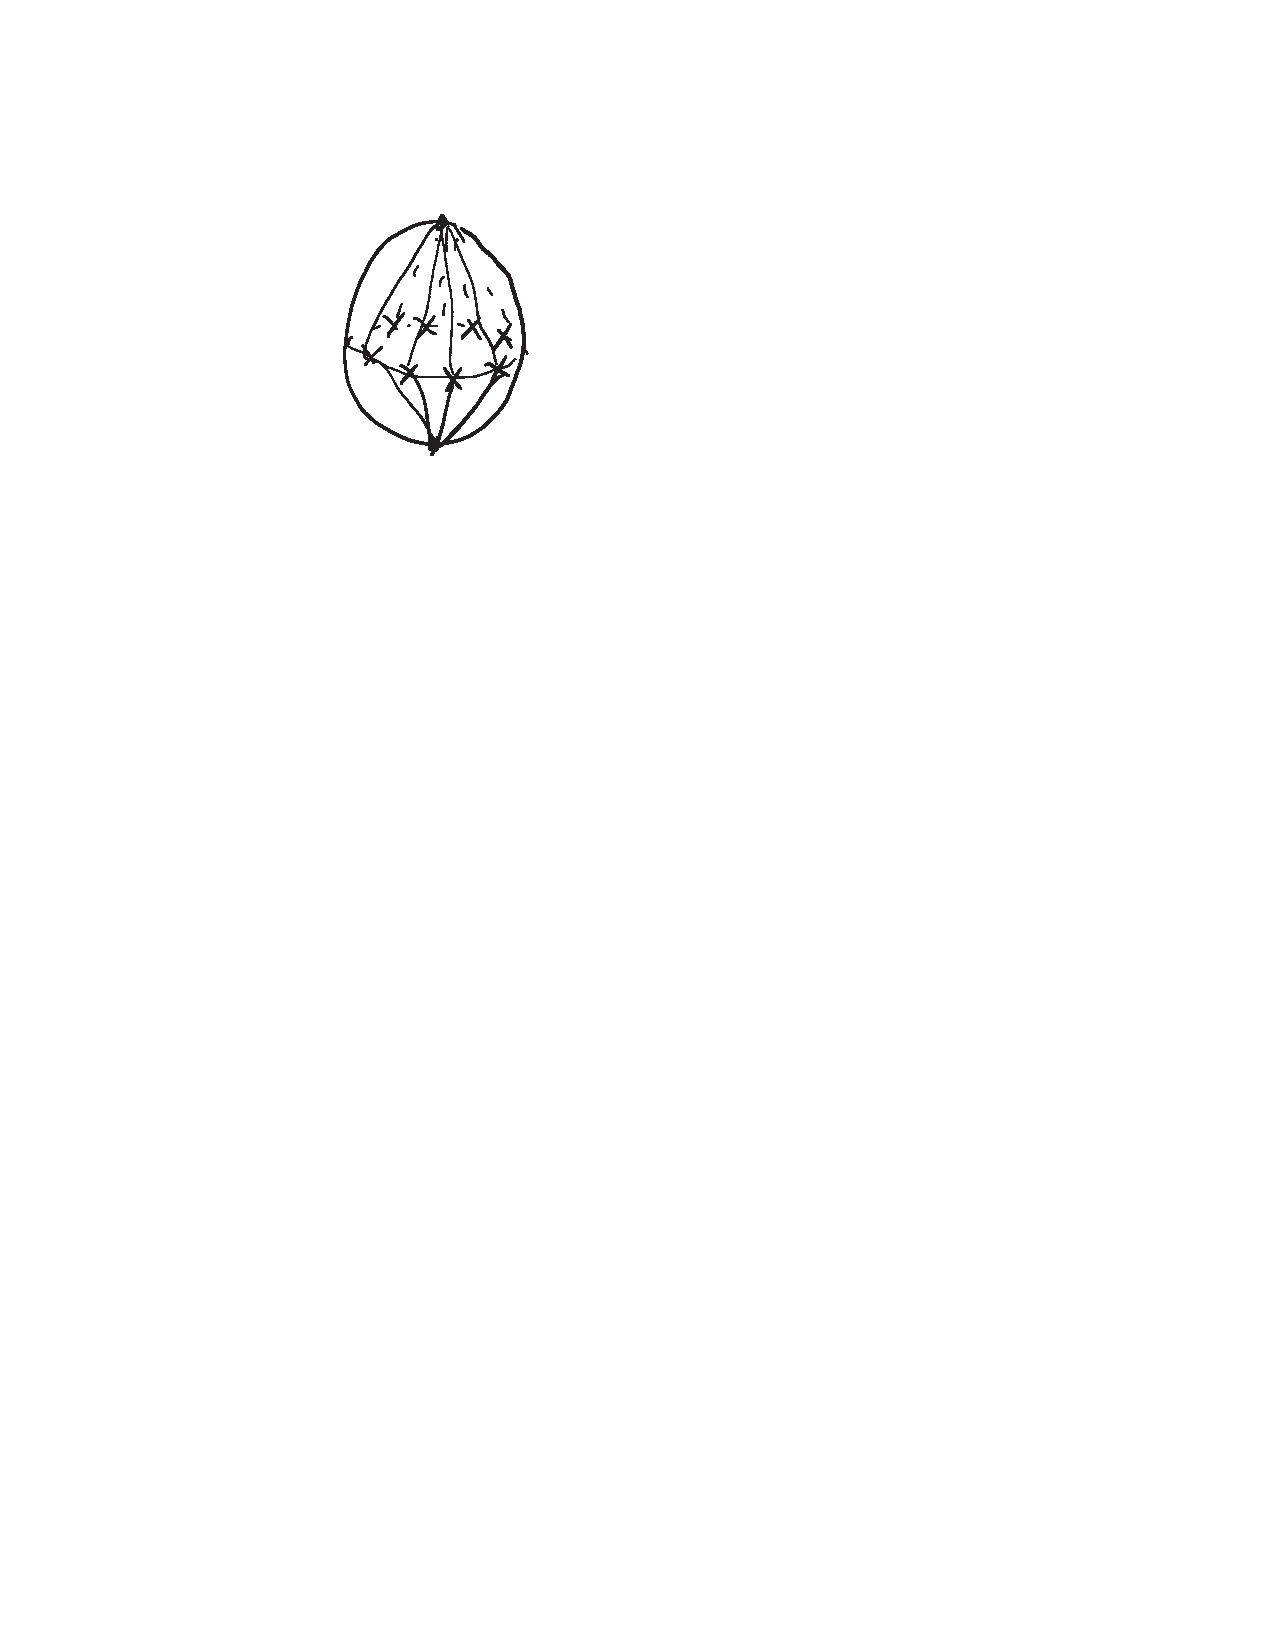
\includegraphics[width=0.5\textwidth]{2011-02-14_Diagram_001}\end{center}
          These points distribute themselves along the equator of $\mathbb P^1$.  Adding points at the poles, there are $2 + d$ vertices, $d + d + d = 3d$ edges, and $2d$ faces, which gives us 2. This is what happens ``downstairs'' (in the projected curve onto $X = \mathbb P^1$).\\
          Upstairs, there is an induced triangulation:
          \begin{itemize}
            \item vertices: $d + d + d = 3d$
            \item edges: $3d^2$
            \item faces: $2d^2$
          \end{itemize}
          Then the Euler characteristic is $E = 3d- 3d^2 + 2d^2 = 3d - d^2 = d(3 - d)$.  Then $g = \frac12(d - 1)(d - 2)$.
        \end{enumerate}
      \item Let $C$ be a smooth curve of degree $d$.  Assume the coefficient of $z^d$ is not zero.  Divide by that coefficient, giving $f(x, y, z) = z^d - a_1(x, y) z^{d-1} + \cdots \pm a_d(x, y)$.  Homogenous polynomial $\implies$ $a_i(x, y)$ is degree $i$ in $x$ and $y$.  Then drop $z$ by projection onto $\mathbb P^1(x, y)$.

        Fix $(x_0, y_0)$.  View $z^d - a_1(x_0, y_0) z^{d-1} + \cdots \pm a_d(x_0, y_0) = 0$ as a polynomial of degree $d$ in $z$.  Typically this has $d$ roots, but for some values of $(x, y)$, there are $d-1$ roots.

        There is a polynomial $\Delta$, discriminant, degree $d(d - 1)$ in $x$ and $y$.  $\Delta = 0$ iff there are less than $d$ roots.  (The discriminant for a quadratic is $b^2 - 4ac$.  It tells you whether or not the polynomial has double roots.)  (Note, if the discriminant has only simple roots, then the claim above (that there are only $d$ or $d - 1$ roots at any point) is intuitively/geometrically true.)

        Triangulate $X = \mathbb P^1$ by putting vertices at these $d(d - 1)$ points.  For $\mathbb P^1$, the Euler characteristic is $2$.  Pulling the triangulation up, the Euler characteristic is approximately $2d$ (everything gets multiplied by $d$).  However, we placed the vertices at the $d(d - 2)$ points where there are $d - 1$ roots.  Then the Euler characteristic is $2d - d(d - 1) = 3d - d^2$.
    \end{enumerate}
\end {document}
